\documentclass[10pt, two column]{article}

\usepackage[utf8]{inputenc}
\usepackage{textcomp}
\usepackage{hyperref}
\usepackage{amsmath}
\usepackage{amsthm}
\usepackage{graphicx}
\usepackage{epigraph}
\usepackage{enumitem}
\usepackage{mathptmx}
\usepackage{times}
\usepackage{listings}

\theoremstyle{definition}
\newtheorem{definition}{Definition}[section]

\lstset{
  basicstyle=\ttfamily,
  columns=fullflexible,
  breaklines=true
}

\title{\huge Phi, a modern successor to Verilog}
\author{Mohamed Gaber \and Aya Elnaggar}
\date{May 2019}

\begin{document}

\onecolumn
\maketitle
\begin{abstract}
\textbf{Objective:} Develop a new hardware description language focusing on the register transfer level with concise and clear semantics based on the Verilog Hardware Description Language. Method: The language was designed with semantic and syntactic cues from the C and Swift programming languages and the Verilog Hardware Description Language. Conclusion: The language design more accurately reflects the design of the hardware, is less tolerant of ambiguity and is syntactically closer to modern programming languages. Clinical Impact: Because of its simplicity, the language is a great introductory language to digital logic design. It also offers an easy transition for those already writing Verilog. The simpler design should also allow for more robust tooling.\newline
     
\textbf{Index Terms—hardware description language, verilog, electronic design automation, language design}

\end{abstract}

\tableofcontents
\newpage
\twocolumn

\section{Introduction}
{\huge\textbf T}he Verilog Hardware Description Language was created in 1984 by Philip Moorby and his team at Gateway Design Automation (now a part of Cadence Design Systems \cite{threeDecadesofHDL} steadily gained popularity and is currently the dominant modeling language for application-specific integrated circuit (ASIC) design in addition to its considerable presence in field programmable logic array (FPGA) design \cite{foster_2016}. Verilog itself was standardized in 1996 as IEEE Std. 1364-1995 \cite{IEEEstandardHDLbasedonVer_1996}, which was updated multiple times until its latest version in 2006, Std. 1364-2005\cite{IEEEstandardforVerilogHDL_2006}. 
\newline

Unfortunately, Verilog is a deeply flawed language by modern standards, being ambiguous and unsafe, with “classic” missteps such as leniency with conversions and other missteps that come from not being designed for purely synthesizable hardware. Many research projects have aimed to design new hardware description languages, however they have tended to either be embedded languages within syntactically alien languages or completely unique research projects that discards parts or most of Verilog’s semantics.\newline

This report explores the design and implementation of a new hardware description language based on widely-acknowledged Verilog best practices that does not discard Verilog’s legacy, yet does away with ambiguity, redundancy and makes the syntax closer to the C family of programming languages to appeal to a new generation of hardware designers.

\section{Motivation}
\subsection{Issues with Verilog}
While Verilog was initially designed for both simulation and synthesis \cite{threeDecadesofHDL}, 
it has been developed solely for simulation for a good portion of its life, and thus has an unfortunate tendency of providing for the description impossible hardware \cite{borrione1992three}.\newline

As such, Verilog had come to rely on a concept of a “synthesizable subset”\cite{synthesizableSubset_2017}, as there are a lot of features in Verilog that simply cannot be replicated in actual hardware. This is not only limited to constructs that are clearly for simulation, some hardware constructs in Verilog are simply impossible in real life. For example: 
\begin{lstlisting}
always @ (posedge ACLK or negedge ACLK or posedge ARESETn)
\end{lstlisting}

While not inherently faulty, this hardware is not synthesizable as registers tend to only support a single sensitivity, and any more sensitivities would have to be detected using separate hardware. However, as Verilog relies on its “triggers” feature to model sensitive registers, synthesizers are left to deal with this, some, such as the open source Yosys tool, outright rejecting it.\newline

The concept of a “synthesizable subset” is not limited to irreplicable hardware, however, as there are constructs that are purely for simulation. Perhaps the most obvious example is the utilization of software function calls. Verilog has a laundry list of function calls that are executed at run time, which are almost impossible to replicate in hardware. It is part of a larger problem with Verilog in general, and it is its general lack of a divide between software and hardware constructs. Between imaginary hardware and literal software, the standard has largely cemented Verilog’s position as a simulation language with limited synthesis capabilities.

\subsection{Newer Languages}
These issues have led to various attempts to create other languages to succeed Verilog. These have ranged from university research projects such as University of California at Berkeley’s Chisel\cite{Chisel_2012}, UC at Santa Cruz’s Pyrope\cite{Pyrope}and industry veteran Jon Decaluwe’s MyHDL\cite{MyHDLmanual_2018}.\newline 

An interesting phenomenon is the development of what has been referred to as an “embedded” hardware description language. At their core, these are libraries written for other programming languages with a desirable syntax and relies on the use of operator overloading and functions to approximate a hardware description language. These do have the advantage of avoiding the syntactic design work, but have the disadvantage of muddying the language semantics with the hardware description semantics, and alienating Verilog users with its syntax.\newline 

The most prominent example of this is the Chisel hardware description language. Chisel is embedded into the Scala Programming Language\cite{scalaOverview2004}, and uses its package management for modularization.  It has the added benefit of having testbenches be written in an existing software programming language, which makes more sense as testbenches are, by nature, procedural constructs. Scala addresses a lot of existing problems with Verilog.  A very clear and very separate distinction between run-time and compile-time logic by relying on Scala’s robust type system.; some types are reserved for run-time logic and others are preserved compile-time logic. Chisel’s strong typing also helps the language determine the correct course of action in matters such as arithmetic vs. logical shifting, a problem so proliferative in Verilog that it introduced opaque compiler constructs such as \$signed to help rectify the issue. Regardless, these advantages arguably do not outweigh the inherent drawbacks of the use of an embedded language.\cite{Chisel_2012}\newline

Some others are supersets of Verilog, the most popular being SystemVerilog, which has become so popular in recent years that a synthesizable subset of System Verilog has been conflated with Verilog itself. System Verilog introduces powerful new software features for verification, which has paid off as SystemVerilog continues to be the most popular language for simulation and verification of both ASIC and FPGA designs\cite{foster_2016}.Some new hardware constructs to be more explicit, however as a superset of Verilog it continues to inherit many of its problems.\cite{IEEEstandardforVerilog_UHD_S_VL_2005}\newline

There are some languages that are built from scratch, including Pyrope and Lucid, however they tend to ignore some syntactic familiarites Verilog has to C entirely in favor of their own syntax: Pyrope especially looks particularly removed from Verilog syntactically and semantically even more so\cite{Pyrope}. That is not to say these languages do not have their benefits, as Pyrope prides itself on being fully synthesizable. For newcomers this might not formulate a problem, however as the industry is very dependent on Verilog, it can be rather difficult to move to a completely different paradigm.\newline

\subsection{Design Goals for Phi}
Phi’s primarily design goal is the creation of a hardware description language that is syntactically and semantically more concise than Verilog, yet one that embraces Verilog’s legacy by continuing to be ultimately similarly structured semantically and syntactically to the Verilog Hardware Description Language.\newline 

This can be boiled down to four essential goals:
% Alphabetical
\begin{enumerate}[label=\alph*)]
\item Unambiguous
\item Fully synthesizable
\item Closer to the C family of languages to appeal to newcomers
\item Close to Verilog semantically to not alienate its veterans.
\end{enumerate}

These goals should be able to culminate in a language that is simple to use, more efficient in a production environment, easier to learn by newcomers but not a jarring transition for existing Verilog users.

\section{Design Process}
As a successor to Verilog with inspirations from the C-family of languages, it was clear Phi was going to be developed as a derivative language rather than one that is designed from scratch. Semantically, the obvious choice was Verilog, as it could then be cut to size from the verbosity. Syntactically, the Swift Programming Language was chosen, as it had a modern expressive yet concise take on C and C++’s syntax \cite{swiftProgLang2019}.\newline
 
Many elements, such as the general code organization, has been retained from Verilog. There is a single top module that instantiates other submodules, where this module is then used for simulation or synthesis.\newline 

\begin{figure}
  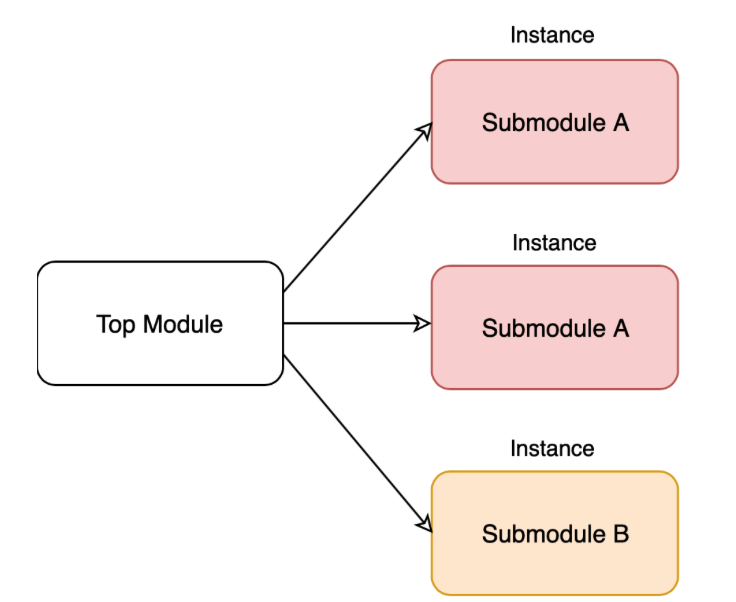
\includegraphics[width=\linewidth]{module_hierarchy.png}
  \caption{\textit{Module Hierarchy in Verilog and Phi}}
  \label{fig:module_hierarchy}
\end{figure}

Perhaps the most significant semantic departure for Phi is the lack of a software type system. A type system has never particularly made sense in hardware, as all values are bit-vectors where each wire can only be off or on. In other hardware description languages, it seems that trajectory is to introduce stricter typing. While this does make sense in software, in hardware it is arguably worse. In Phi, the operators decide how the bitvectors should behave. Arithmetically, they behave as integers. Inspired by ECMAScript \cite{ECMAScript_2018}, the one operation where the sign matters on bitvectors, the right shift, was migrated to Phi, where it has a similar behavior.\newline

This has also affected Phi’s syntax import from Swift, as Swift’s typing syntax did not translate very well. Swift used var and let to denote declaration and an extra identifier or type expressions. The concept of types doesn't exist in Phi, and thus Phi reverted to the C-style declarations of type then variable name.\newline 

The “types” in said situation refer to “Var”, “Register” and “Wire”, where the former indicates software expressions evaluated at compile/elaboration time, and the latter two are hardware constructs to be simulated or synthesized. This is to satisfy the goal of a strict software/hardware divide.\newline

This strict software/hardware divide also allows for initially more cumbersome definitions in Verilog to become less so, such as declaring arrays of components. What required the Verilog generate block- essentially metaprogramming, is now idiomatic to Phi as now components can now be declared in arrays and hooked separately. For example:\newline

\begin{lstlisting}
genvar i;
for (i = 0; i < 10; i = i + 1) begin
    Example example(
        .a(a[i]),
        .b(b[i]),
        .q(q[i]),
        .r(r[i])
    );
end

Example example[10];
for i in 0..9 {
    example[i](
        a: a[i],
        b: b[i],
        q: q[i],
        r: r[i]
    );
}
\end{lstlisting}
\begin{center}
\textit{Instantiating an array of modules in Verilog and Phi}
\end{center}

What does have the potential to create a difference in a hardware description language is bus width safety. Unlike Verilog, Phi is strict about bus widths, and these requirements may not be waived. Phi will not automatically extend nor prune expressions to fit a specific bus width. This rule is universal: for example, even an expression as trivial as \textbf{1b1 + 1b1 + 1b1} would be incorrect, as the first two result in a two-bit wide expression that would be incompatible with the third one-bit wide expression. Also, all conditions in Phi, whether for if statements, ternary expressions or the newly introduced mux expression, which is similar to a switch statement that takes a comma-delimited list of expressions instead.\newline 

Incidentally, numbers in Phi are encouraged to specify a width and a base, for example \textbf{30xABC} would declare a 30-bit integer with the unsigned decimal value of 48879. Numbers declared without a width and base are 32-bit and decimal by default, but their use is discouraged. Phi had initially intended on disallowing integers without explicit widths and bases, but it came at a syntactic verbosity cost that was simply too cumbersome, and thus the concept was discarded.\newline 

Another significant semantic departure that was decided upon at the very beginning involved blocking vs non-blocking assignments. Verilog had introduced the idea of procedural modeling of hardware: namely that a developer may be able to simply write down some lines of code and these lines of code should be synthesizable. The confusion has always been one of the greatest sources of bewilderment with the Verilog Hardware Description Language. Multiple languages have attempted to address this issue to various degrees of success. Initially, Phi went for MyHDL’s approach, which is just to be also able to treat wires as signals similar to VHDL, and give registers a \textbf{.next} property that act in lieu of a non-blocking assignment.\newline

Initially, Phi has adopted this approach, although its flaws had soon become readily apparent. The flaws were not with the signal approach in particular, rather, it was the ideal of synthesizing the connections of registers from a synchronous procedural block itself. The flexibility of procedural blocks has proven too much for many synthesizers, and unless one is to read the manual of specific synthesizer and study it very well, synthesis of procedural blocks has since descended into a case by case basis. This is deeply undesirable for a language that has the goal “fully synthesizable,” as it would take only one module that would fail to synthesize to fail to meet this goal.\newline

Phi has thus transitioned to a model where procedural blocks are only used to model combinational logic. Registers are instead modeled in a very structural manner, where they have wire properties \textbf{(.data, .reset, .clock and .enable)}. These wires can be connected to a similar manner to a what a D flip-flop would be connected in actual hardware, which is straightforward to both visualize and synthesize. Designers can continue to use asynchronous blocks for combinational logic, but the actual writing to the register is black-boxed to the designer, as they should be at the register-transfer level. Phi does not support lower level modeling of hardware. Being that registers now with a specific synchronicity regardless of procedural blocks, registers can now no longer be assigned to with blocking or non-blocking semantics: using the = operator sets the value of the register when reset.\newline

\begin{figure}
  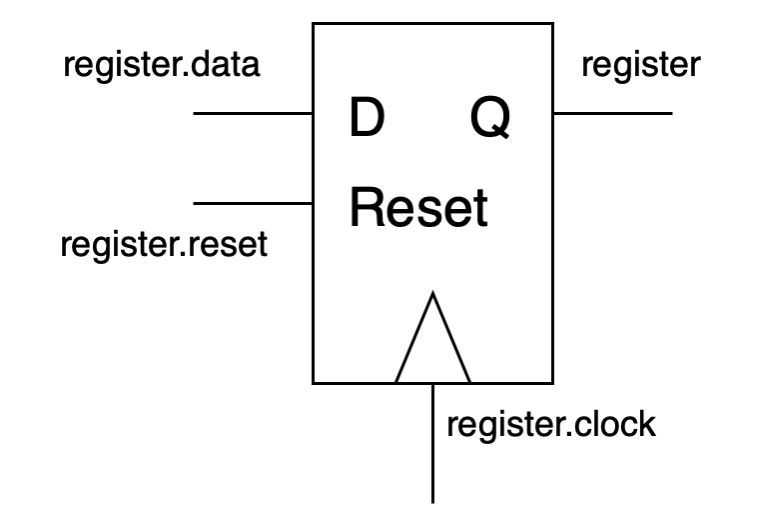
\includegraphics[width=\linewidth]{register_in_phi.png}
  \caption{\textit{A Register in Phi. Registers in Phi are based on D flip-flops in actual hardware.}}
  \label{fig: a register in Phi.}
\end{figure}

This culminated in the creation of the async block. At a basic level, the \textbf{async} block is similar to the \textbf{always\_comb} block in Verilog, however with the key distinction being that in Phi, \textbf{async} blocks always assign to wires and all of: assignment to registers, assignment to variables, declarations are strictly prohibited, as they exist only to relate wires combinationally. Phi async blocks\newline 

\begin{lstlisting}
async {
   if (y) {
       a = 32b0;
   } else {
       a = 32xBAD;
   }
}
\end{lstlisting}
\begin{center}
\textit {An async block in Phi. y and a are both wires.}
\end{center}

That said, the name async is a leftover from an early design phase in the development of procedural blocks where a procedural block would use the defunct keyword \textbf{sync}. At this point, it might be confusing and there various options being explored to change it.\newline

Outside of the \textbf{async} block, however, Phi has done away with procedural semantics entirely. Phi embraces the concept of perpetuity in hardware. As actual hardware, with the possible exception of FPGA, do not have an “initial” state, such statements are not synthesizable. Thus, it is imperative that all elements of Phi execute in perpetuity (including the async block, as it effectively counts as one statement).\newline

There are other numerous small semantic tweaks. This includes namespacing, which allows modules to exist under a namespace. It allows multiple modules to exist with the same name, so long as they are properly namespaced. On the topic of modules, Phi also defines interfaces in the vein of Java’s 
interfaces and Swift’s protocols, which would define a set of input ports that instantiators would have to drive and a set of output ports that the compliant module would have to drive. This is especially useful when developing intellectual properties for use with buses, which do tend to mandate certain port names and/or widths.\newline

Syntactic tweaks are also numerous: as shown in Figure 2, the C-style for loop has been abandoned in favor of the for loop used in more modern C-family languages. The C-style for loop has generally been frowned upon for its opacity and syntactic aberrance. The while and do while loops have been eliminated. Ranges have had their syntax slightly tweaked, now using the .. operator from Perl and Ruby. This was more of an implementation detail than a meaningful change and a revert to Verilog’s : may occur if future field testing of the language proves the double dots too jittery a transition.\newline

\begin{lstlisting}
module Counter(
   clock: @clock Input,
   reset: @resetLow Input,
   output: Output[31..0]
) {
   Register[31..0] store = 32b0;
   store.data = store &+ 1;
   output = store.data;
}
\end{lstlisting}
\begin{center}
\textit{A typical Phi module under this design}
\end{center}

\section{Implementation}

As this project aims mainly to design Phi rather than implement it, implementation of Phi was mainly kept to simple, well-documented tools.\newline

Phi was initially implemented in the classic duo of Unix compiler implementation: Lex and Yacc. Because these tools are a part of the UNIX® specification \cite{openGroupBaseSpecif_2018}, supporting these tools would have made the compiler very portable across multiple platforms. However, this has introduced many limitations stemming from the fact the compiler was written in C++, which is not a part of the Unix specification. While it is possible to have implemented this compiler in C, time constraints and the team’s own development experience could not accommodate that, and it was quickly switched over to GNU Flex and GNU Bison, as both tools do have limited support for C++. \newline

Bison’s C++ support is rather impressive: generating a full “Parser” class that fully encapsulates its functionality. Flex did not fare as well, generating code that was invalid when operated in C++ mode. Flex was thus used in C mode, i.e. with no generation of a “Scanner” class to go with Bison’s Parser class, meaning multithreading of multiple inputs would prove difficult. Another more minor issue is the lack of Unicode support, which while might not seem important, can be interesting to support for some east Asian markets. A different tool named ReFlex is currently being examined, which touts Unicode support and generates C++ code \cite{reflex}.\newline

Initially, there were two methods of implementation to consider: direct translation and constructing a tree. The former was easier to implement, but as it inflated the size of a file with many dependents (namely, the yacc file), it also added a bottleneck during the compilation phase. Additionally, it was very difficult to perform the static checking Phi promises in this structure, so it was quickly abandoned.\newline

The static checking is itself one of the more challenging areas in the implementation. As Phi modules are instantiatable by Verilog modules and vice versa, Phi modules need to be able to algebraically verify width expressions as the value of the expression can only be known after Phi’s compiler has concluded if the expression incorporates parameters.\newline

The other form involved tree generation. This has not yet been implemented due to the complexity involved. 

\section{Testing}
Phi was tested using about 100 modules. All of that exhaustive testing contributed to: 
\begin{itemize}
	\item Taking some design decisions 
	\item Locating issues
	\item Pinpointing the current major challenges 
\end{itemize} 

One of those design decisions is how to represent the multiplexer using Phi language. As with Verilog, there are many, but Phi adds one more in the form of the mux expression, which is unique to Phi. This does add some slight redundancy. The second design decision taken is that the polarity to every port has to be written. This does ensure consistency at the cost of relative verbosity.\newline
 
There were not many implementation issues in Phi, and the only issue that was discovered by testing was fixed. That issue was that having two right square brackets after one another. That should not be considered as an syntax error whether there is white space between them or not. However, our compiler previously was very sensitive to that, as two consecutive right square brackets used to be a token.\newline

\begin{lstlisting}
Q_reg.data = [sinr,Q_reg[3..1]];
\end{lstlisting}
\begin{center}
\textit{Right square brackets issue. Notice how the part in bold used to be a token.}
\end{center}


The biggest challenge facing Phi compiler is error reporting. As a limitation of the implementation technologies (GNU Flex and GNU Bison), error reports are vague and often in the wrong place. It is not that accurate- but this should be rectified with the aforementioned improvement of tooling.

\section{Comparison}
Comparing Phi with other HDLs  was essential to evaluate the language. Phi was thus compared with:
\begin{itemize}
	\item Verilog
	\item MyHDL
	\item Chisel 
	\item Lucid
\end{itemize}

Verilog does maintain a single advantage: it is very obvious for the user to get for example what is always happening because of \textbf{always @} block, as the sensitivity list is very explicit.Phi however requires a read of the specification to learn that registers act like D flip-flops, and the issue is somewhat compounded by the fact Phi  has also some shorthand notation that may confuse those looking at new codebases.\newline

MyHDL benefits from using the high level language Python\cite{MyHDLmanual_2018}. MyHDL clearly differentiates between combinational blocks and sequential blocks using \textbf{@always\_comb} and \textbf{@always\_seq} \cite{MyHDLmanual_2018}, similar to SystemVerilog’s \textbf{always\_comb} and \textbf{always\_seq}. MyHDL and Phi are similar due to their common ancestry in Verilog. Both require specifying width for inputs, outputs and registers. Giving an initial value for registers is also required for both languages.\newline

However, MyHDL is syntactically very far away from Verilog. Not only because of using high level language but also the way of thinking of hardware is very different, as it utilizes the concept of signals introduced in VHDL\cite{VHDLmanual_2009}. MyHDL has a keyword Signal that represents all signals in a block, and it focuses on the signal going into and out of the block rather than the block itself. \cite{MyHDLmanual_2018}\newline

\begin{lstlisting}
Signal(intbv(0)[3:0])
 @always(Clock.posedge)
 def logic1():
  Q.next = concat(Q[2:0],SI)
 return logic1
\end{lstlisting}
\begin{center}
\textit{MyHDL code}
\end{center}

Chisel provides more representation of what happens inside the block and how every building block interacts with one another. That is very clear in the example in the following figure which shows a 4-bit serial in and serial out shift register. Like MyHDL, Chisel and Phi do retain some similarities: both require specifying width for inputs, outputs and registers. Giving an initial value for registers are also required for both languages.\newline

\begin{lstlisting}
val delays = RegInit(VecInit(initValues))
 for (i <- 3 to 1 by -1) {
   delays(i) := delays(i - 1)
 }
 delays(0) := io.SI
 io.SO := delays(3)
\end{lstlisting}
\begin{center}
\textit{Chisel code}
\end{center}

However, it is much more verbose to represent all of that kind of information. Additionally, Chisel is structured much more like the Java family of languages, with very heavy object orientation that makes code generally very verbose. While Phi does support namespacing, it is not as rigid as Chisel.\newline

Lucid is even more precise than Chisel in representing what is going on in the block. Because it does not only show how the building blocks interact together but it also shows what are the building blocks very explicitly. In the example given in the following snippet, Lucid mentions \textbf{dff pipe[4]} which is very easy to infer as to mean 4 D flip-flops. Lucid also makes the representation of dff  very clear by using .d and .q to represent the inputs and outputs. This is clearly advantageous over Phi as Phi currently has to introduce an exception to allow Registers to be readable and not writable, which violates the language design principle of things looking similarly behaving similarly. That said, Phi’s Register type is not explicitly a D flip-flop, so it is possible adding .d and .q would further compound the confusion.\newline

\begin{lstlisting}
dff pipe[4] (.clk(clk));
   var i;
     always {
       pipe.d[0] = serial_in;
       serial_out = pipe.q[3];
       for (i = 1; i < 3; i++)
         pipe.d[i] = pipe.q[i-1];
\end{lstlisting}
\begin{center}
\textit{Lucid code}
\end{center}

Despite the fact that all of that very detailed information is very good to be known and clear for the user, it is, much like Chisel, very verbose in terms of the code that need to be written. One other limitation found is that all datatype names have to be written in lowercase \cite{withMojoAndLucid_2017}. That limitation is not there in Phi. Overall however, Lucid is the closest language to Phi, but some key differences do keep them apart.

\section{Conclusion}
While there are a few design considerations remaining to iron out, Phi has developed into a language that is reminiscent of Verilog, yet one that has taken on its own identity.\newline

Phi remains simple and attractive to newcomers, and yet any industry veteran should be able to quickly realize its design around informal Verilog best practices.\newline

At this point, research on Phi is geared towards the implementation of the compiler to be ready for field testing by the start of the Spring 2019 semester.\newline

The simpler design of Phi should also allow Phi to integrate more simply with other design tools, and it is planned for the reference compiler to implement features to integrate with electronic design automation tools in the near future.

\section*{Appendix}
The full Phi specification as of the time of writing is available at: \url{https://github.com/donn/Phi/tree/fb2f405fabe5aab215ea39b6ee823b55c34efd12/Specifications}

\section*{Acknowledgment}
We would like to acknowledge Professor Mohamed Shalan of the American University in Cairo for his consistent input on the language, and Professor Sherif Aly for supervising and advising the research project.

\bibliography{refs}
\bibliographystyle{ieeetr}

\end{document}
